%\documentclass[handout]{beamer}
\documentclass{beamer}

\usepackage{amsmath,amsfonts,amssymb,graphicx} 
\usefonttheme[onlymath]{serif}
% use article-like math letters, from http://tex.stackexchange.com/questions/34265/how-to-get-beamer-math-to-look-like-article-math


\newcommand\bi{\begin{itemize}}
\newcommand\ei{\end{itemize}}
\newcommand\simMC{\stackrel{\scriptscriptstyle{MC}}{\sim}}


% from genPomp ms
\newcommand\T{\mathbb{T}}
\newcommand\transmission{\mathcal{T}}
\newcommand\observation{\mathcal{G}}
\newcommand\observationTree{genetic tree}
\newcommand\descendents{h}
\newcommand\sequenceLabel{q}
\newcommand\tInit{t_{0}}
\newcommand\tRoot{t_{\mathrm{root}}}
\newcommand\tEnd{t_{\mathrm{end}}}
\newcommand{\circled}[1]{
  \kern-0.4em \raisebox{.1pt}{\textcircled{\raisebox{-.9pt} {#1}}}
}

\usepackage{natbib}
\usepackage{url}
\usepackage{ulem}
\renewcommand\emph[1]{{\it #1}} % the ulem package redefines \emph
\renewcommand\em{\it} % the ulem package redefines \emph

\usepackage{xcolor}
\definecolor{olive}{rgb}{0.3, 0.4, .1}
\definecolor{dgreen}{rgb}{0.,0.6,0.}
\definecolor{gold}{rgb}{1.,0.84,0.}
\definecolor{JungleGreen}{cmyk}{0.99,0,0.52,0}
\definecolor{BlueGreen}{cmyk}{0.85,0,0.33,0}
\definecolor{RawSienna}{cmyk}{0,0.72,1,0.45}
\definecolor{Magenta}{cmyk}{0,1,0,0}

\usepackage{graphicx} % Allows including images
%\usepackage{booktabs} % Allows the use of \toprule, \midrule and \bottomrule in tables
\mode<presentation> {

\usetheme{Madrid}

%%\setbeamertemplate{footline}[frame number]
\setbeamertemplate{footline}{
  \hfill%
  \usebeamercolor[fg]{page number in head/foot}%
  \usebeamerfont{page number in head/foot}%
  \setbeamertemplate{page number in head/foot}[framenumber]%
  \usebeamertemplate*{page number in head/foot}\kern1em\vskip2pt%
}

\setbeamertemplate{navigation symbols}{} 

}

\newcommand\myemph[1]{{\textbf{#1}}}
\newcommand\enumerateSpace{\hspace{2mm}}
\usepackage{amssymb}
\newenvironment {myitemize} {
                 \begin{list}{\textcolor{black}{$\bullet$} \hfill}
%                 \begin{list}{\textcolor{blue}{{\small{$\blacktriangleright$}}} \hfill}
                 {\setlength{\labelwidth}{0.3 cm}
                  %\setlength{\leftmargin}{0em}
                  \setlength{\leftmargin}{0.15cm}
                  \setlength{\itemindent}{0.15cm}
                  \setlength{\labelsep}{0cm}
                  \setlength{\parsep}{0.2 ex}
%                  \setlength{\itemsep}{0.25 cm}
                  \setlength{\itemsep}{1 mm}
%                   \setlength{\itemsep}{0.0 cm}
      \setlength{\topsep}{0.0cm}}} %space between title and 1st item
   {\end{list}}

\newcommand\MainFigureBmScaling{1}
\newcommand\MainFigureMeaslesScaling{2}
\newcommand\MainFigureMeaslesSlice{3}

%\newcommand\SuppFigureMeaslesSharedSlice{\eic{TODO}}

\newcommand\SuppSecGeneralization{S1}
\newcommand\SuppSecThmI{S3}
\newcommand\SuppSecThmII{S4}
\newcommand\SuppSecMemoryEfficient{S10}
\newcommand\SuppSecAdaptedSimulation{S2}
\newcommand\SuppSecBM{S5}
\newcommand\SuppSecMeasles{S6}
\newcommand\SuppSecMeaslesNbhd{S7}
\newcommand\SuppSecMeaslesGammaSlice{S8}
%\newcommand\SuppSecMeaslesReducedNoise{S9}
\newcommand\SuppSecLorenz{S9}
%\newcommand\SuppSecMeaslesIJ{S11}

%\newcommand\AssumptionBivb{\ref{B:unconditional:mix}(b)}
%\newcommand\AssumptionBiva{\ref{B:unconditional:mix}(a)}
\newcommand\comma{{\hspace{-0.25mm},\hspace{-0.2mm}}}
\newcommand\termStart{\dagger}
%\newcommand\termStart{\circ}

\newcommand\amplitude{a}
\newcommand\meanBeta{{\bar\beta}}
\newcommand\cohort{c}
\newcommand\birth{b}


%\title{Locally weighted island filters for partially observed spatiotemporal systems}

\title{Island filters for partially observed spatiotemporal systems}


%%%%%%%%%%%%%%%% START OF USER DEFINITIONS %%%%%%%%%%%%%%%5

\newcommand\siOnly[1]{} %% redefined for the supplement
\newcommand\msOnly[1]{#1} %% redefined for the supplement

%\newcommand\tif{\mathrm{tif}}
\newcommand\inputSpace{\rule[-1.5mm]{0mm}{4.7mm}}
\newcommand\firstLineSpace{\rule[0mm]{0mm}{4mm}}
\newcommand\lastLineSpace{\rule[-2.5mm]{0mm}{4mm}}

\newcommand\gravity{G}

\newcommand\AIRSIF{ASIF-IR}
\newcommand\TIF{BIF}
\newcommand\centersum{\Delta}
\newcommand\mediumint{\resizebox{2.8mm}{!}{$\displaystyle \int$}}
%\newcommand\Bsize{|B|}
\newcommand\Bsize{b}
%\newcommand\UnitSet{\mathbb{U}}
%\newcommand\TimeSet{\mathbb{N}}
\newcommand\TimeSet{\mbox{TimeSet should now be ObsTimeSet or ProcTimeSet}}
\newcommand\UnitSet{1{\mycolon}\Unit}
\newcommand\ObsTimeSet{1{\mycolon}\Time}
\newcommand\ProcTimeSet{0{\mycolon}\Time}
%\newcommand\spaceTime{\mathbb{S}}
\newcommand\spaceTime{\UnitSet\times\ObsTimeSet}
%\newcommand\unitTimeSubset{\mathbb{C}}
\newcommand\unitTimeSubset{B}
%\newcommand\adapted{\rho}
\newcommand\adapted{\gamma}
\newcommand\myeqref[1]{[\ref{#1}]}
\newcommand\tif{{}}
\newcommand\girf{\mathrm{girf}}
\newcommand\gir{G}
\newcommand\altAltTime{m}


\newcounter{wwii}
\setcounter{wwii}{1}
\newcommand\wwiiStep{\makebox[8mm][l]{\arabic{wwii}.}\stepcounter{wwii}}
\newcounter{wwiiResample}
\newcounter{wwiiAncestor}
\newcounter{wwiiPredict}
\newcounter{wwiiFilter}

\newcounter{asii}
\setcounter{asii}{1}
\newcommand\asiiStep{\makebox[8mm][l]{\arabic{asii}.}\stepcounter{asii}}
\newcounter{girasif}
\setcounter{girasif}{1}
\newcommand\girasifStep{\makebox[8mm][l]{\arabic{girasif}.}\stepcounter{girasif}}
\newcounter{asiiResample}
\newcounter{asiiAncestor}
\newcounter{asiiPredict}
\newcounter{asiiFilter}
\newcounter{girasifResample}
\newcounter{girasifAncestor}
\newcounter{girasifPredict}
\newcounter{girasifFilter}


% package used by default for Overleaf
%\usepackage[utf8]{inputenc}

%% code macros
%\newcommand\slot[1]{\code{#1}}
%\newcommand\class[1]{class `\code{#1}'}
\newcommand\code[1]{\texttt{#1}}
\usepackage{url}

\newcommand\W{W}
\newcommand\V{V}
\newcommand\ASindex{[\Unit]}
\newcommand\simulation{\mathrm{sim}}

%\renewcommand\baselinestretch{1.3}
%\usepackage{showkeys}
%\usepackage[numbers,sort&compress]{natbib}
%\bibliographystyle{apalike}

%\usepackage{natbib}
%\bibliographystyle{plainnat}
%\bibliographystyle{dcu}
%\usepackage{url}

\newcommand\pstep[1]{{\bf #1}}
\newcommand\qsp{\rule{0mm}{1mm}\hspace{4mm}}
\newcommand\plusStrut{\rule{0mm}{1.2mm}}

%% basic POMP definitions
\newcommand\Xspace{{\mathbb X}}
\newcommand\Yspace{{\mathbb Y}}
%\newcommand\Thetaspace{{\Theta}}
\newcommand\Thetaspace{\R^{\Thetadim}}
\newcommand\Xunitspace{{\scriptsize{\mathcal X}}}
\newcommand\Yunitspace{{\tiny{\mathcal Y}}}
\newcommand\hatTheta{\widehat{\Theta}}
\newcommand\Xdim{{\mathrm{dim}}(\Xspace)}
\newcommand\Ydim{{\mathrm{dim}}(\Yspace)}
%\newcommand\Thetadim{{\mathrm{dim}}(\Thetaspace)}
\newcommand\Thetadim{P}
\newcommand\thetadim{p}
\newcommand\timeSet{{\mathbb T}}
\newcommand\data[1]{#1^*}

\newcommand\unitSpecific{\hspace{0.1mm}\mathrm{us}}
\newcommand\shared{\hspace{0.15mm}\mathrm{sh}}

%% for particle filters
\newcommand\unit{u}
\newcommand\altUnit{\tilde u}
\newcommand\Unit{U}
\newcommand\rep{i}
\newcommand\altIsland{\tilde i}
\usepackage[mathscr]{euscript}
\newcommand\Rep{\mathcal{I}}
\renewcommand\time{n}
\renewcommand\vec[1]{\boldsymbol{#1}}
\newcommand\altTime{\tilde n}
\newcommand\Time{N}
\newcommand\Np{J}
\newcommand\np{j}
\newcommand\altNp{k}
\newcommand\altAltNp{\tilde j}
\newcommand\resampleIndex{r}
\newcommand\unitWeight{w}


%% for ASIF and HIPPIE
\newcommand\IF{\mathrm{A}}  % adapted simulation
\newcommand\IP{\mathrm{P}}  % adapted proposal
%\newcommand\GR{\mathrm{GR}}  % GIR resample 
%\newcommand\GP{\mathrm{GP}}  % GIR proposal 
\newcommand\GR{\mathrm{IR}}  % intermediate resample 
\newcommand\GP{\mathrm{IP}}  % intermediate proposal 
\newcommand\resample{\mathrm{R}} % this would have been F before
\newcommand\proposal{\mathrm{P}} 
\newcommand\LCP{\mathrm{P}}  % local prediction 
\newcommand\LCF{\mathrm{F}}  % local filter 

%% for GIR
%\newcommand\Lookahead{L}
%\newcommand\lookahead{\ell}
\newcommand\Ninter{S} %% number of intermediate timepoints
\newcommand\ninter{s}
%\newcommand\Nguide{K} %% number of lookahead particles
%\newcommand\nguide{k}
%\newcommand\lookaheadEnd{\time\oplus \Lookahead}
%\newcommand\lookaheadEnd{\min(\time+\Lookahead,\Time)}
\newcommand\guideFunc{g}
%\newcommand\VtoTheta{{\overleftarrow{V}}}
%\newcommand\thetaToV{{\overrightarrow{V}}}
%\newcommand\VtoTheta{{\overline{V}}}
%\newcommand\thetaToV{\underline{V}}
%\newcommand\thetaToV[1]{\stackrel{\rightarrow}{\mathrm{v}}_{\hspace{-0.5mm}#1}\!}
%\newcommand\VtoTheta[1]{\stackrel{\leftarrow}{\mathrm{v}}_{\hspace{-0.5mm}#1}\!}
\newcommand\thetaToV{\stackrel{\rightarrow}{\mathrm{v}}\!}
\newcommand\VtoTheta{\stackrel{\leftarrow}{\mathrm{v}}\!}
%\newcommand\thetaToV[1]{\stackrel{\rightarrow}{\mathrm{v}_{#1}}\!}
%\newcommand\VtoTheta[1]{\stackrel{\leftarrow}{\mathrm{v}_{#1}}\!}
\newcommand\npgir{\np}
\newcommand\Npgir{\Np}
\newcommand\Nguide{G}

%% for all iterated filtering algorithms
\newcommand\Nit{M}
\newcommand\nit{m}


%% customized math macros
\newcommand\prob{\mathbb{P}}
\newcommand\E{\mathbb{E}}
\newcommand\dd[1]{\mathrm{d}{#1}}
\newcommand\given{{\,\vert\,}}
\newcommand\equals{{{\,}={\,}}} 
\newcommand\myequals{\hspace{0.5mm}{=}\hspace{0.5mm}}
\newcommand\myto{{\;:\;}}
\newcommand\seq[2]{{#1}\!:\!{#2}}
\newcommand\mydot{{\,\cdot\,}}
\newcommand\cp[2]{N_{\mathrm{#1}\mathrm{#2}}}
\newcommand\giventh{{\hspace{0.5mm};\hspace{0.5mm}}}
%\newcommand\normal{{\mathrm{Normal}}}
\newcommand\normal{\mathcal{N}}
\newcommand\argequals{{\,=\,}}
\newcommand\lags{c}
\newcommand\maxlag{\overline{c}}
\newcommand\nlfList{C}
\newcommand\bigO{\mathcal{O}}
\newcommand\loglik{\lambda}
\newcommand\loglikMC{\MC{\loglik}}
\newcommand\R{\mathbb{R}}
\newcommand\param{\,;}
\newcommand\mycolon{{\hspace{0.6mm}:\hspace{0.6mm}}}
\newcommand\MC[1]{#1^{\,\mbox{\tiny MC}}}
%\newcommand\EMC{\MC{\E}}
\newcommand\EMC{{\E}}
\newcommand\Var{\mathrm{Var}}
\newcommand\var{\Var}
\newcommand\Cov{\mathrm{Cov}} 
\newcommand\cov{\Cov}
\newcommand\iid{\mathrm{iid}}
%\newcommand\dist{\mathrm{dist}}
\newcommand\dist{d}
\newcommand\transpose{\top}

\newcommand\gnsep{,}

\def\lik{L}
\def\loglik{\ell}

%% THEOREM-LIKE ENVIRONMENTS
\usepackage{amsthm}
\newtheorem{prop}{Proposition}
%\newtheorem{theorem}{Theorem}
%\newtheorem{lemma}{Lemma}
%\newtheorem{example}{Example}
\newtheorem{remark}{Remark}
\newtheorem{cor}{Corrolary}
%\newtheorem{fact}{Fact}  
\newtheorem{assumption}{Assumption}
\newtheorem{assumptionB}{Assumption}
\newtheorem{procedure}{Procedure}
\renewcommand\theassumption{A\arabic{assumption}}
\renewcommand\theassumptionB{B\arabic{assumptionB}}

%\usepackage{float}
%\floatstyle{ruled}
%\newfloat{textbox}{t}{tbx}
%\floatname{textbox}{Box}
%\renewcommand\thetextbox{\arabic{textbox}}


%% FOR PSEUDOCODE SETUP
\newcommand\mystretch{\rule[-2mm]{0mm}{5mm} }   
\newcommand\asp{\hspace{4mm}}

%%%%%%%%%%%%%%%% END OF USER DEFINITIONSS %%%%%%%%%%%%%%%5


\newcommand\PartOfBoundOffDiagonal{3\efourB+4(K + \dmax)\,\efive}
\newcommand\boundOffDiagonal{\efourA + \PartOfBoundOffDiagonal}
\newcommand\K{K^\prime}
\newcommand\ThmOneVarBound{Q^{4b} \, \Unit\Time  \big(\altb + \etwo \, (\Unit\Time-\altb) \big)}


\newcommand\BvConstant{\mathcal{C}_0}
\newcommand\dmax{d_{\max}}
\newcommand\boundLemma{\efourB+(K+d_{\unit,\time})\efive}
\newcommand\boundLemmaUniform{\efourB+(K+\dmax)\efive}


%\newcommand\altB{\tilde{B}}
\newcommand\altB{C}
%\newcommand\el{\epsilon_\ell}
\newcommand\el{\epsilon}   %%% epsilon for Thm 1
%\newcommand\eone{\epsilon_1}
%\newcommand\eone{\epsilon^{}_{\!\mathrm{\ref{A1}}}}
\newcommand\eone{\epsilon^{}_{\!\mathrm{A1}}}
%\newcommand\eone{\epsilon^{A}_{1}}
%\newcommand\etwo{\epsilon^{}_{\!\mathrm{\ref{A:unconditional:mix}}}}
\newcommand\etwo{\epsilon^{}_{\!\mathrm{A4}}}
%\newcommand\altb{\tilde{b}}
\newcommand\altb{c}
\newcommand\Ai{
\begin{assumption}\label{A1}
There is an $\eone>0$ and a collection of neighborhoods $\{B_{\unit\comma\time}\subset A_{\unit\comma\time}, \unit\in 1\mycolon\Unit,\time\in 1\mycolon\Time\}$ such that, for all  $\unit$, $\time$, $\Unit$, $\Time$,  any  bounded real-valued function $|h(x)|\le 1$, and any value of $x_{B^c_{\unit\comma\time}}$, 
%\begin{equation}
\begin{eqnarray}
\nonumber
&& \hspace{-12mm} \Bigg| \int h(x_{\unit\comma\time}) f_{X_{\unit\comma\time}|Y_{B_{\unit\comma\time}},X_{B^c_{\unit\comma\time}}}(x_{\unit\comma\time}\given  \data{y}_{B_{\unit\comma\time}}, x_{B^c_{\unit\comma\time}}) \, dx_{\unit\comma\time}
\\
\siOnly{\label{eq:weak_coupling2}}
\msOnly{\nonumber}
&& \hspace{-3mm} - \int h(x_{\unit\comma\time})f_{X_{\unit\comma\time}|Y_{B_{\unit\comma\time}}}(x_{\unit\comma\time}\given \data{y}_{B_{\unit\comma\time}})
\, dx_{\unit\comma\time}
\Bigg| \hspace{1mm} < \hspace{1mm} \eone.
%\end{equation}
\end{eqnarray}
\end{assumption}
}

\newcommand\Aii{
\begin{assumption}\label{A1b}
For the collection of neighborhoods in Assumption~\ref{A1}, with $B^+_{\unit\comma\time}=B^{}_{\unit\comma\time}\cup (\unit,\time)$, there is a constant $\Bsize$, depending on $\eone$ but not on $\Unit$ and $\Time$, such that
\begin{equation}
\nonumber
\sup_{\unit\in 1:\Unit, \, \time\in 1:\Time} \big| B^+_{\unit\comma\time}\big| \le \Bsize.
\end{equation}
\end{assumption}
}

\newcommand\Aiii{
\begin{assumption}\label{A2}
There is a constant $Q$ such that, for all $\unit$ and $\time$, $\Unit$ and $\Time$,
\begin{equation}
\nonumber
Q^{-1} <f_{Y_{\unit\comma\time}|X_{\unit\comma\time}}(\data{y}_{\unit\comma\time}\given x_{\unit\comma\time}) < Q
\end{equation}
\end{assumption}
}

\newcommand\Aiv{
  \begin{assumption}\label{A:unconditional:mix}
    There exists $\etwo > 0$ such that the following holds.
    For each $\unit, \time$, a set $\altB^{}_{\unit\comma\time} \subset (1\mycolon U)\times(0\mycolon N)$ exists such that $(\altUnit, \altTime) \notin \altB_{\unit\comma\time}$ implies $B_{\unit\comma\time}^+ \cap B_{\altUnit\comma\altTime}^+ = \emptyset$ and
      \begin{equation} 
\siOnly{\label{eq:A:unconditional:mix}}
\msOnly{\nonumber}
        \big| f_{X_{B^{+}_{\altUnit\comma\altTime}}|X^{}_{B^{+}_{\unit\comma\time}}} - f_{X_{B^{+}_{\altUnit\comma\altTime}}} \big|
        < \etwo \, f_{X_{B^{+}_{\altUnit\comma\altTime}}}
      \end{equation}
      Further, there is a uniform bound $|\altB_{\unit\comma\time}| \le \altb$.
\end{assumption}
}

\newcommand\TheoremI{
\begin{theorem}  \label{thm:tif}
Let $\MC{\loglik}$ denote the Monte Carlo likelihood approximation constructed by {\TIF}.
Consider a limit with a growing number of islands, $\Island\to\infty$, and suppose assumptions~\ref{A1},~\ref{A1b} and~\ref{A2}.
There are quantities $\el(\Unit,\Time)$ and $V(\Unit,\Time)$, with bounds $|\el|<\eone Q^{2}$ and $V < Q^{4\Bsize} \, U^2 N^2$, such that
\begin{equation}
\label{th1:lik:bound}
\Island^{1/2}\big[ \MC{\loglik}-\loglik-\el\Unit\Time \big]  \xrightarrow[\Island \rightarrow \infty]{d} \normal\big[0,V\big],
\end{equation}
where $\xrightarrow[\Island \rightarrow \infty]{d}$ denotes convergence in distribution and $\normal[\mu,\Sigma]$ is the normal distribution with mean $\mu$ and variance $\Sigma$.
If additionally Assumption~\ref{A:unconditional:mix} holds, we obtain an improved variance bound
\begin{equation}
\label{th1:lik:bound2}
V < \ThmOneVarBound.
\end{equation}
\end{theorem}
}


%%% 2222222222222222222222


%\newcommand\ethree{\epsilon^{}_{\mathrm{\ref{B1}}}}
\newcommand\ethree{\epsilon^{}_{\mathrm{B1}}}
%\newcommand\efourA{\epsilon^{}_{\mathrm{\ref{B:unconditional:mix}}}}
\newcommand\efourA{\epsilon^{}_{\mathrm{B4}}}
%\newcommand\efourB{\epsilon^{}_{\mathrm{\ref{B:temporal:mix}}}}
\newcommand\efourB{\epsilon^{}_{\mathrm{B5}}}
%\newcommand\efive{\epsilon^{}_{\mathrm{\ref{B:girf}}}}
\newcommand\efive{\epsilon_{\mathrm{B6}}}

\newcommand\Bi{

\begin{assumptionB}\label{B1}
  There is an $\ethree>0$ and a collection of neighborhoods $\{B_{\unit\comma\time}\subset A_{\unit\comma\time}, \unit\in 1\mycolon\Unit,\time\in 1\mycolon\Time\}$ such that the following holds for all $\unit$, $\time$, $\Unit$, $\Time$, and any bounded real-valued function $|h(x)|\le 1$\emph{:} if we write $A=A_{u,n}$, $B=B_{u,n}$, $f_{A}(x_A) = f_{Y_{A}|X_{A}}(\data y_{A}|x_A)$, and $f_{B}(x_B) = f_{Y_{B}|X_{B}}(\data y_{B}|x_B)$,
%\begin{equation}
\begin{eqnarray}
\nonumber
%\label{asif:eq:weak_coupling2}
&&\hspace{-7mm}
\left| 
\int \hspace{-1mm} h(x)
\left\{
\frac{
  \E_{g} \! \big[ 
    f_{A}\big(X_{A}^P\big) f_{X_{u,n}|X_{A^{[n]}},\vec X_{n-1}} \big(x | X_{A^{[n]}}^P, \vec X_{n-1}\big) 
  \big]
} {
  \E_{g} \! \big[f_A\big(X_A^P\big)\big]
} - 
\right.
\right.
\\
\nonumber
&& 
\siOnly{\hspace{20mm}}
\hspace{-6.5mm} 
% - \hspace{-1mm} 
\siOnly{\hspace{2mm}}
\left.
\left.
\frac{
  \E_{g} \! \big[
    f_{B}\big(X_{B}^P\big) f_{X_{u,n}|X_{B^{[n]}},\vec X_{n-1}}\big(x | X_{B^{[n]}}^P, \vec X_{n-1}\big) \big] 
} {
  \E_{g} \! \big[f_B\big(X_B^P\big)\big]
} 
\!
\right\}
\!
dx
\right| \hspace{0mm} < \hspace{0mm} \ethree.
%\end{equation}
\end{eqnarray}
\end{assumptionB}
}

\newcommand\Bii{
\begin{assumptionB}\label{B1b}
The bound $\sup_{\unit\in 1:\Unit,\time\in 1:\Time} \big| B^+_{\unit\comma\time}\big| \le \Bsize$ in Assumption~\ref{A1b} applies for the neighborhoods defined in Assumption~\ref{B1}. 
This also implies there is a finite maximum temporal depth for the collection of neighborhoods, defined as
\begin{equation}
\nonumber
\dmax=\sup_{(\unit,\time)}\hspace{1mm} \sup_{(\altUnit,\altTime)\in B_{\unit,\time}}|\time-\altTime|.
\end{equation}
\end{assumptionB}
}

\newcommand\Biii{
\begin{assumptionB}\label{B2} Identically to Assumption~\ref{A2}, 
$Q^{-1} <f_{Y_{\unit\comma\time}|X_{\unit\comma\time}}(\data{y}_{\unit\comma\time}\given x_{\unit\comma\time}) < Q$.
\end{assumptionB}
}

\newcommand\BivA{
\begin{assumptionB}\label{B:unconditional:mix}
Define $g_{{X}_{A}|{X}_{B}}$ via \myeqref{eq:g}.
Suppose there is an $\efourA$ such that the following holds.
For each $\unit, \time$, a set $\altB^{}_{\unit\comma\time} \subset (1\mycolon U)\times(0\mycolon N)$ exists such that $(\altUnit, \altTime) \notin \altB_{\unit\comma\time}$ implies $B_{\unit\comma\time}^+ \cap B_{\altUnit\comma\altTime}^+ = \emptyset$ and
%      \begin{eqnarray} 
%\label{eq:B:unconditional:mix:1}
\begin{equation}
\nonumber
\big| 
   g^{}_{{X}^{P}_{B^{}_{\altUnit\comma\altTime}}{X}^{P}_{B^{}_{\unit\comma\time}}} 
   - g^{}_{{X}^{P}_{B^{}_{\altUnit\comma\altTime}}} \, g^{}_{{X}^{P}_{B^{}_{\unit\comma\time}}} 
\big|
<
%&\hspace{-3mm}<\hspace{-3mm} & 
%\\
%&&\hspace{-30mm}
(1/2) \, \efourA \, \,  g^{}_{{X}^{P}_{B^{}_{\altUnit\comma\altTime}}} \, g^{}_{{X}^{P}_{B^{}_{\unit\comma\time}}}
%\\
%\label{eq:B:unconditional:mix:2}
\end{equation}
\begin{eqnarray}
\nonumber
\big|
g^{}_{X^P_{B^{}_{\altUnit\comma\altTime}}|\vec{X}_{0:\Time}} 
\, g^{}_{X^P_{B^{}_{\unit\comma\time}}|\vec{X}_{0:\Time}} 
-
g^{}_{X^P_{B^{}_{\altUnit\comma\altTime}},X^P_{B^{}_{\unit\comma\time}}|\vec{X}_{0:\Time}}
\big|
&&
%&\hspace{-3mm}<\hspace{-3mm}& 
\\
\nonumber
%&&\hspace{-30mm}(1/2) \, \efourA \, \, 
&&\hspace{-30mm} < (1/2) \, \efourA \, \, 
 g^{}_{X^P_{B^{}_{\altUnit\comma\altTime}},X^P_{B^{}_{\unit\comma\time}}|\vec{X}_{0:\Time}}
      \end{eqnarray}
      Further, there is a uniform bound $|\altB_{\unit\comma\time}| \le \altb$.
\end{assumptionB}
}
\newcommand\BivB{
\begin{assumptionB}\label{B:temporal:mix}
There is a constant $K$ such that, for any set $D\subset (\UnitSet)\times(n{\mycolon}n-d)$ and for all $\time\ge K+d$, $\vec{x}^{(1)}_{\time-d-K}$, $\vec{x}^{(2)}_{\time-d-K}$, and all $x^{}_{D_n}$,
\begin{eqnarray}
\nonumber
&&\hspace{-6mm} \big|
g^{}_{{X}_{D}|\vec{X}_{\time-d-K}}(x^{}_{D}\given\vec{x}^{(1)}_{\time-d-K})
-
g^{}_{{X}_{D}|\vec{X}_{\time-d-K}}(x^{}_{D}\given\vec{x}^{(2)}_{\time-d-K})
\big|
\\
\nonumber
&& \siOnly{\hspace{10mm}} \hspace{4mm}
< 
\efourB  \,  \,
g^{}_{{X}_{D}|\vec{X}_{\time-d-K}}(x^{}_{D_n}\given\vec{x}^{(1)}_{\time-d-K})
\end{eqnarray}

\end{assumptionB}
}

\newcommand\Bv{
\begin{assumptionB}\label{B:girf}
Let $h$ be a bounded function with $|h(x)|\le 1$. 
Let $\vec{X}^{\GR}_{\time,\Ninter,\np,\island}$ be the Monte Carlo quantity constructed in ASIF-IR, conditional on $\vec{X}^{\IF}_{\time-1,\Ninter,\island}=\vec{x}^{\IF}_{\time-1,\Ninter,\island}$.
There is a constant $\BvConstant(\Unit,\Time,\Ninter)$ such that, for all $\efive^{}>0$ and $\vec{x}^{\IF}_{\time-1,\Ninter,\island}$, whenever the number of particles satisfies $J > \BvConstant(\Unit,\Time,\Ninter)/\efive^{4}$,
\begin{equation}
\nonumber
\hspace{-0.5mm}
\left|  
\, 
  \EMC\Big[ 
    \frac{1}{\Np} \sum_{\np=1}^{\Np} h(\vec{X}^{\GR}_{\time,\Ninter,\np,\island}) 
   \Big] \!
-  \E_g \! \big[h(\vec{X}_\time)\given \vec{X}_{\time-1}=\vec{x}^{\IF}_{\time-1,\Ninter,\island}\big] 
\right| \!
< \efive^{}.
\end{equation}
\end{assumptionB}
}

\newcommand\Bvi{
\begin{assumptionB}\label{B:XG_XA_ind}
For $1\leq \time \leq N$, the Monte Carlo random variable $X^A_{\time,i}$ is independent of $w^M_{\unit,\time,i,j}$ conditional on $X^A_{\time-1,i}$.
\end{assumptionB}
}


\newcommand\TheoremII{
\begin{theorem}  \label{thm:asif}
Let $\MC{\loglik}$ denote the Monte Carlo likelihood approximation constructed by ASIF-IR, or by ASIF since this is the special case of ASIF-IR with $\Ninter=1$.
Consider a limit with a growing number of islands, $\Island\to\infty$, and suppose assumptions~\ref{B1},~\ref{B1b}, \ref{B2}, \ref{B:temporal:mix}, \ref{B:girf} and~\ref{B:XG_XA_ind}. 
Suppose the number of particles $\Np$ exceeds the requirement for~\ref{B:girf}.
There are quantities $\el(\Unit,\Time)$ and $V(\Unit,\Time)$ with $|\el|<
Q^2\ethree + 2 Q^{2\Bsize}\big(\boundLemma\big)$
and $V<Q^{4\Bsize}\Unit^2\Time^2$ 
such that
\begin{equation}
\siOnly{\label{th:asif:lik:bound}}
\msOnly{\nonumber}
\Island^{1/2}
  \big[ 
    \MC{\loglik}-\loglik-\el\Unit\Time 
  \big]  
  \xrightarrow[\Island \rightarrow \infty]{d} 
  \normal\big[ 0,V \big].
\end{equation}
If additionally Assumption~\ref{B:unconditional:mix} holds, we obtain an improved rate of
\begin{equation}
\siOnly{\label{th:asif:lik:bound2}}
\msOnly{\nonumber}
V < Q^{4\Bsize}\Time\Unit
\big\{ c + \big(\boundOffDiagonal \big) \big(\Time\Unit-c\big)
\big\}
\end{equation}
\end{theorem}
}



\begin{document}

\begin{frame}
  
\begin{center}
  {\Large\bf Inference for metapopulation dynamics}

%% ABSTRACT: Microbial populations can demonstrate highly nonlinear, partially observable, stochastic dynamics. Parameter estimation and model criticism are inferential challenges which are tractable using modern methods applicable to general low-dimensional ecological models. Collections of interacting ecosystems at different locations raise additional challenges associated with high-dimensional Monte Carlo inference. Questions arise about when it is necessary to develop models for dynamic coupling between metapopulations, and if so how to carry out inference in this setting. We seek general-purpose methods that allow scientists to ask and answer questions for metapopulation dynamics in the context of scientifically useful models. We present recent progress and ongoing developments.


\vspace{2mm}

Edward Ionides\\
University of Michigan, Department of Statistics

\vspace{8mm}

Multiscale Microbial Communities\\
Dynamical Models, Ecology, and One Health\\
February 22, 2022


\hspace{3mm}

Slides are at \url{https://ionides.github.io/talks/imsi22.pdf}
%% 8:15am EST

\vspace{8mm}

Joint work with\\
Kidus Asfaw, Ning Ning, Joonha Park and Aaron King

\end{center}

\end{frame}


\newcommand\challengeSep{\vspace{3mm}}

\begin{frame}{Inference challenges in population dynamics}

  \begin{enumerate}
\item Combining measurement noise and process noise.
\item Including covariates in mechanistically plausible ways.
\item  Continuous time models.
\item  Modeling and estimating interactions in coupled systems.
\item  Dealing with unobserved variables.
\item  \myemph{Modeling spatial-temporal dynamics}.
\item  \myemph{Studying population dynamics via genetic sequence data}.
  \end{enumerate}

  \vspace{3mm}
  
  1--6 are from Bjornstad \& Grenfell ({\it Science}, 2001).\\
  7 is from Grenfell et al ({\it Science}, 2004).\\
  1--5 are largely solved, from a methodological perspective.
  
  
\end{frame}

\begin{frame}{Example: Pre-vaccination measles in England \& Wales}

\vspace{-3mm}

\begin{center}
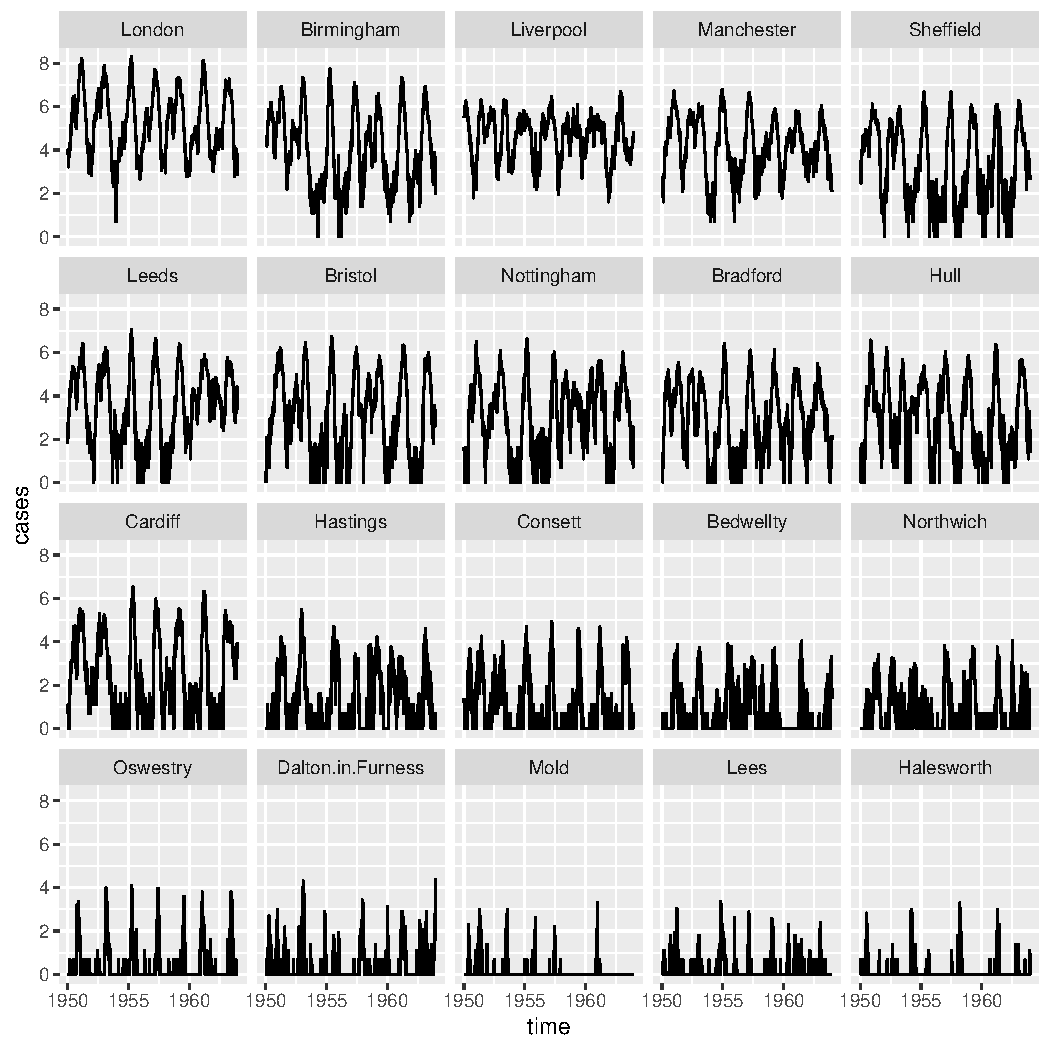
\includegraphics[width=8.5cm]{he10-data.pdf}


\end{center}

\vspace{-2mm}
  
\end{frame}

\begin{frame}{Time series data, panel data \& spatiotemporal data}

  \bi
\item Looking at one unit (town) is \myemph{time series analysis}.

  \item Joint modeling of a few units (say, 2 or 3) is \myemph{multivariate time series analysis}.

\item Analysis of many time series, without consideration of dynamic interactions, is \myemph{panel data analysis}.

\item Allowing for coupling between units, we get \myemph{spatiotemporal analysis}, which in our context is \myemph{metapopulation analysis}.

  \ei
  
Question: When should we avoid inference for spatiotemporal models? When do we need to consider coupling? How?

\end{frame}

\begin{frame}{Desiderata}

  \begin{itemize}
    \item We want to be able to fit arbitrary dynamic models. The limitations should be our scientific creativity and the information in the data.

    \item In practice, that means using \myemph{plug-and-play} methods which need a simulator from the model but not nice closed-form expressions for densities.

    \item We want statistically efficient inference, to extract all the information in the data.

    \item In practice, that means using likelihood-based methods.

      \item  In the time series case, iterated particle filtering (IF2) implemented in the R package \texttt{pomp} enables Masters-level statisticians to do this (\url{https://ionides.github.io/531w22/}). The science may be hard, but the statistics is becoming routine.
      \end{itemize}
  \end{frame}



\begin{frame}{Panel data}

\bi
\item To investigate epidemiological dynamics in multiple cities, one can consider each city independently, perhaps modeling a background immigration rate of infections for each city.

\item \myemph{Decoupling} leads to panel data analysis, by assumption. Iterated filtering methods extend to panel data (Breto et al, {\it Journal of the American Statistical Association}, 2019).

\item We must decide which parameters should be modeled as \myemph{shared} vs \myemph{unit-specific}.

\item The consequences of decoupling are becoming easier to study with the development of statistical inference methods for coupled systems, i.e., metapopulation dynamics.

  \ei

  \end{frame}

\begin{frame}{The curse of dimensionality}

  \bi
  \item
    Particle filter (PF) methods are effective for inference on low-dimensional nonlinear partially observed stochastic dynamic systems. They scale exponentially badly.

\item Extending the successes of particle filter methods from time series data to metapopulation data is becoming possible.

\item Algorithms under consideration:\\
  {\bf
  Bagged filters (BF, IBF)\\
  Ensemble Kalman filter (EnKF, IEnKF)\\
  Guided intermiediate resampling filter (GIRF, IGIRF)\\
  Block particle filter (BPF, IBPF)\\
  }
  
\item Filters estimate latent states and evaluate the likelihood.
\item Each filter has an iterated version which estimates parameters by repeated filtering using stochastic parameter perturbations.

\item These algorithms are all implemented in an R package, \texttt{spatPomp}.
  
  \ei
  
\end{frame}

\begin{frame}{Filtering $U$ units of a coupled measles SEIR model}

\vspace{-3mm}

\begin{center}
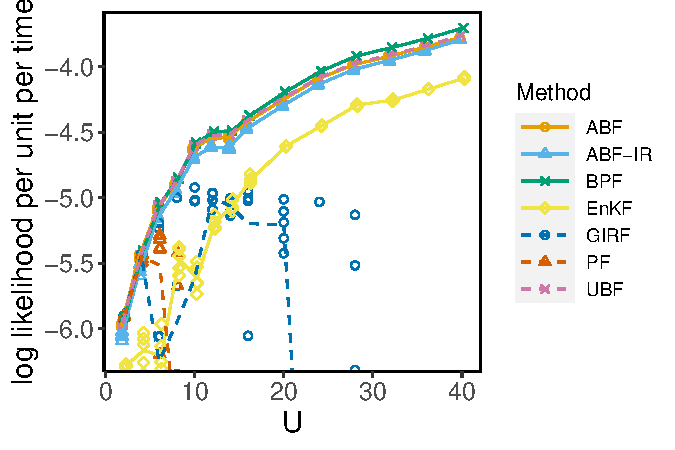
\includegraphics[width=10cm]{mscale_loglik_plot-1.pdf}


\end{center}

\vspace{-2mm}

Simulated data using a gravity model with geography, demography and transmssion parameters corresponding to UK pre-vaccination measles (Ionides et al, {JASA}, 2021).

%\end{center}

\end{frame}

\begin{frame}
\frametitle{$U=40$ units for a coupled measles SEIR model}

\vspace{-2.7mm}

\begin{center}
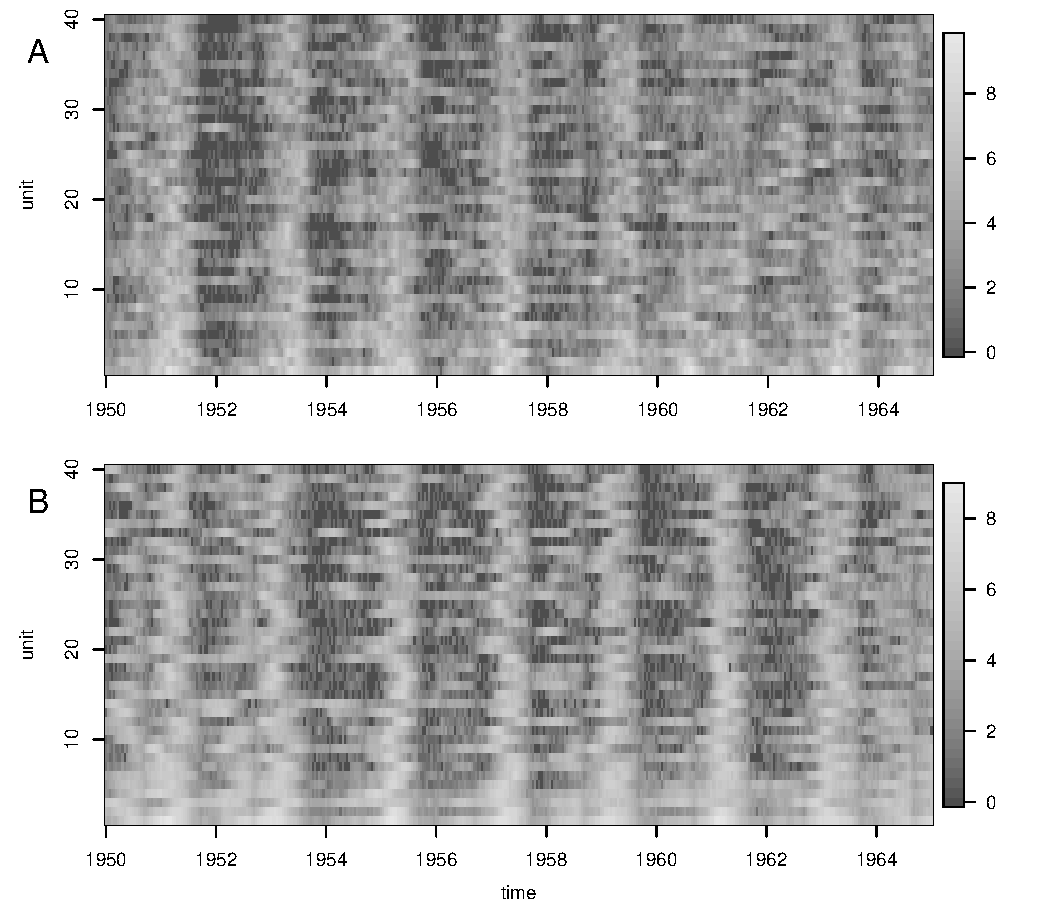
\includegraphics[width=8cm]{slice_image_plot-1.pdf}
\end{center}

\vspace{-3mm}

{\bf A}. Simulated Susceptible-Exposed-Infected-Recovered dynamics coupled with a gravity model (log of biweekly reported cases).

{\bf B}. Measles UK pre-vaccination case reports for the 40 largest cities.




%\end{center}

\end{frame}

\begin{frame}{Parameters for the measles model}
  \bi
\item Seasonal tranmission: mean and amplitude, using school term for contact rate.
  \item Durations of latency and infectious period.
\item Initial values: fraction susceptible, latent and infectious.
\item Cohort effect: all births in an age cohort start school in September.
\item Inhomogenous mixing coefficient.
\item Measurement fraction.
\item Transport model gravity constant.
\item Dynamic noise (process overdispersion).
\item Measurement overdispersion.

\ei

  \end{frame}

\begin{frame}{More on the block particle filter}

\bi
\item BPF worked quickly, easily and reliably on our measles model filtering experiments.

\item This motivated us to develop an IBPF for parameter estimation.
   
\item BPF has theoretical support in some situations (Rebeschini \& Van Handel, {\it Annals of Applied Probability}, 2015).

\item BPF was independently proposed as the ``factored particle filter'' by Ng et al (2002, {\it Proc. 18th Conference on Uncertainty and Artificial Intelligence}) but not widely popularized.

\ei

\end{frame}

\begin{frame}{Particle filter (PF)}

  \begin{columns}
    \begin{column}{0.48\linewidth}
      \begin{center}
      {\bf \textcolor{blue}{Evolutionary analogy}}

      \vspace{5mm}
      
      {\bf Mutation}

      $\downarrow$

      {\bf Fitness}

      $\downarrow$

      {\bf Natural selection}
      
      \end{center}
    \end{column}
     \begin{column}{0.48\linewidth}
      \begin{center}
      {\bf \textcolor{blue}{Particle filter algorithm}}

      \vspace{5mm}
      
      {\bf Predict: stochastic dynamics}

      $\downarrow$

      {\bf Measurement: weight}

      $\downarrow$

      {\bf Filter: resample}
      \end{center}
    \end{column}
  \end{columns}

  \vspace{15mm}
  
    \begin{myitemize}
  \item PF is an evolutionary algorithm with good mathematical properties: an unbiased likelihood estimate and consistent latent state distribution.
  \end{myitemize}

\end{frame}
  
\begin{frame}{Block particle filter (BPF)}

  \begin{columns}
    \begin{column}{0.48\linewidth}
      \begin{center}
      {\bf \textcolor{blue}{Evolutionary analogy}}

      \vspace{5mm}
      
      {\bf Mutation}

      $\downarrow$

      {\bf Fitness\\
      for each chromosome}

      $\downarrow$

      {\bf Natural selection\\
      for each chromosome}

      $\downarrow$

      {\bf Recombine chromosomes}
      
      \end{center}
    \end{column}
     \begin{column}{0.48\linewidth}
      \begin{center}
      {\bf \textcolor{blue}{Block particle filter}}

      \vspace{5mm}
      
      {\bf Predict: stochastic dynamics}

      $\downarrow$

      {\bf Measurement: weight\\
      for each block}

      $\downarrow$

      {\bf Filter: resample\\
      for each block}

      $\downarrow$

      {\bf Recombine blocks}
      \end{center}
    \end{column}
  \end{columns}

  \vspace{5mm}
  
    \begin{myitemize}
    \item Blocks in BPF allow recombination (reassortment of chromosomes in sexual reproduction) in the evolutionary analogy.
    \item Blocks are a partition of the metapopulation units. Our experiments suggest treating each sub-population (i.e., city) as a block.

  \end{myitemize}

\end{frame}

\begin{frame}

\frametitle{Measles likelihood slices for coupling parameter, $G$}

\vspace{-5mm}

\begin{columns}[T] % align columns
\begin{column}{.55\textwidth}
  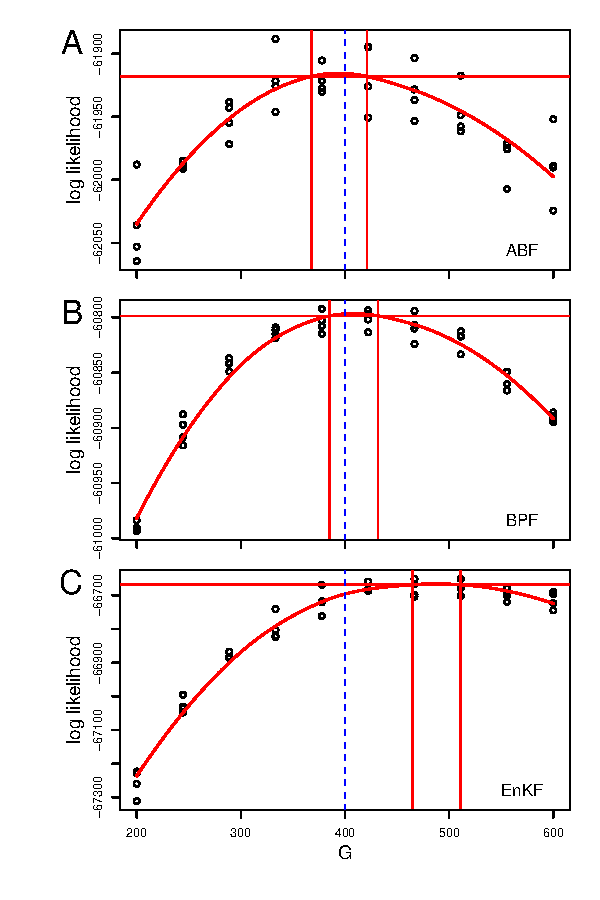
\includegraphics[width=6cm]{slice_combined_plot-1.pdf}
\end{column}
\begin{column}{.52\textwidth}

  \vspace{6mm}
  
  Simulating $15$ year of data from $U=40$ cities for the measles model.
  Slice likelihood, varying $G$ with other paramters fixed at the truth.

  \vspace{3mm}

  {\bf A}. Evaluation using adapted bagged filter (ABF).

    \vspace{3mm}

  {\bf B}. Evaluation using block particle filter (BPF).

    \vspace{3mm}

  {\bf C}. Evaluation using EnKF.

  \vspace{3mm}
  
Results from Ionides et al (2021, {\it JASA}). We computed a slice due to lack of good optimization algorithms to compute a profile.
  
\end{column}
\end{columns}

\end{frame}


\begin{frame}{An iterated block particle filter for parameter estimation}


  \begin{center}
    
  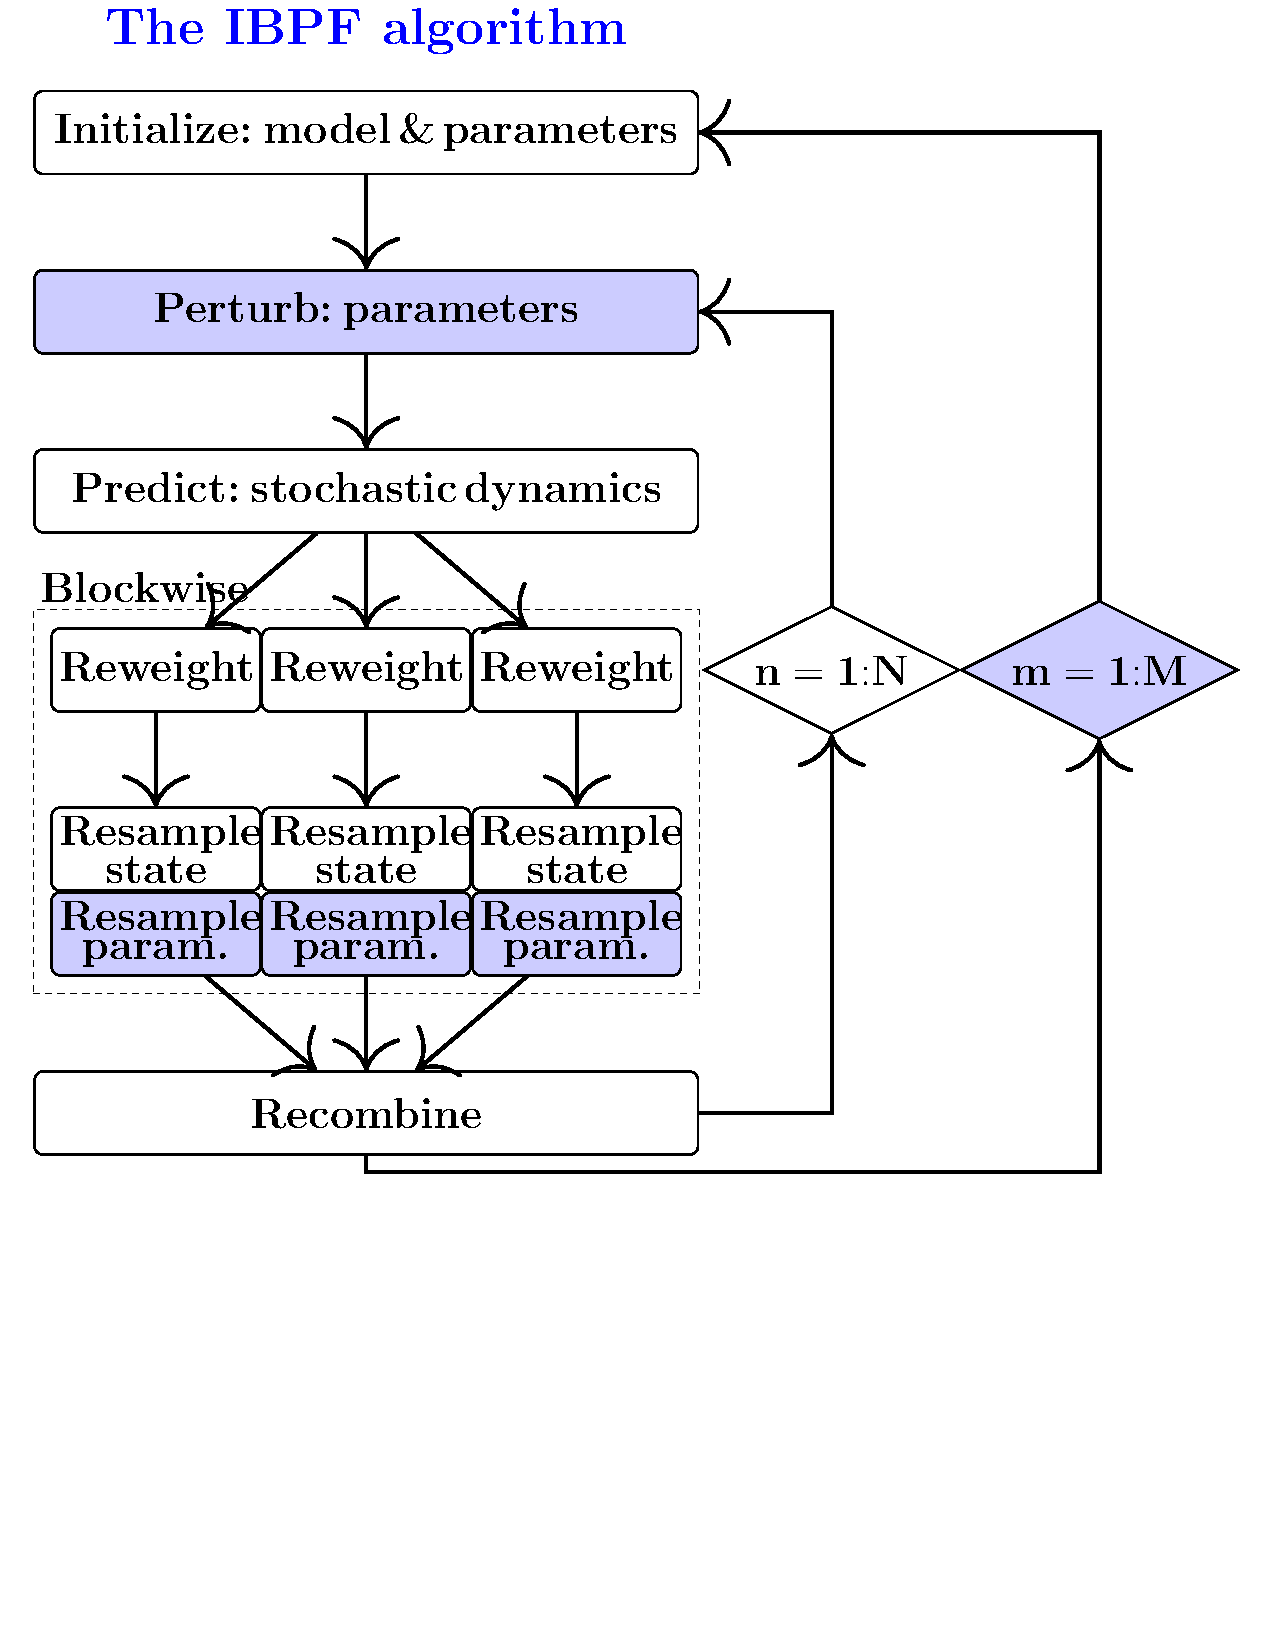
\includegraphics[trim={0 0 0 10mm},clip,width=9cm]{IBPF_workflow.pdf}


  \end{center}
  
\end{frame}


\begin{frame}{Scalability needed for practical inference}

Large numbers of parameters
  \begin{itemize}
  \item  Initial conditions will typically have to be estimated for each unit.
  \item Various dynamic parameters and measurement parameters (e.g., reporting rate) may also need to be unit-specific to obtain a statistical fit to the data.
\item Working with hundreds of estimated parameters raises additional challenges on top of the high-dimensional coupled dynamics.
  \end{itemize}

\vspace{5mm}
  
A moderate numbers of spatial units is enough to open new possibilities.

  \begin{itemize}
  \item As soon as dimension exceeds capabilities of a particle filter (say, $U=5$) we are in situations where likelihood-based inference for general models has been inaccessible.

  \item 10-100 coupled units is our target problem size.

  \item Larger problems will need numerical approximations (e.g., EnKF). Exact Monte Carlo methods help study the effect of these approximations.
    
  \end{itemize}

  \end{frame}
 
    
\begin{frame}{Auto-regression of spatial perturbations for shared parameters}

\vspace{-10mm}

\begin{center}
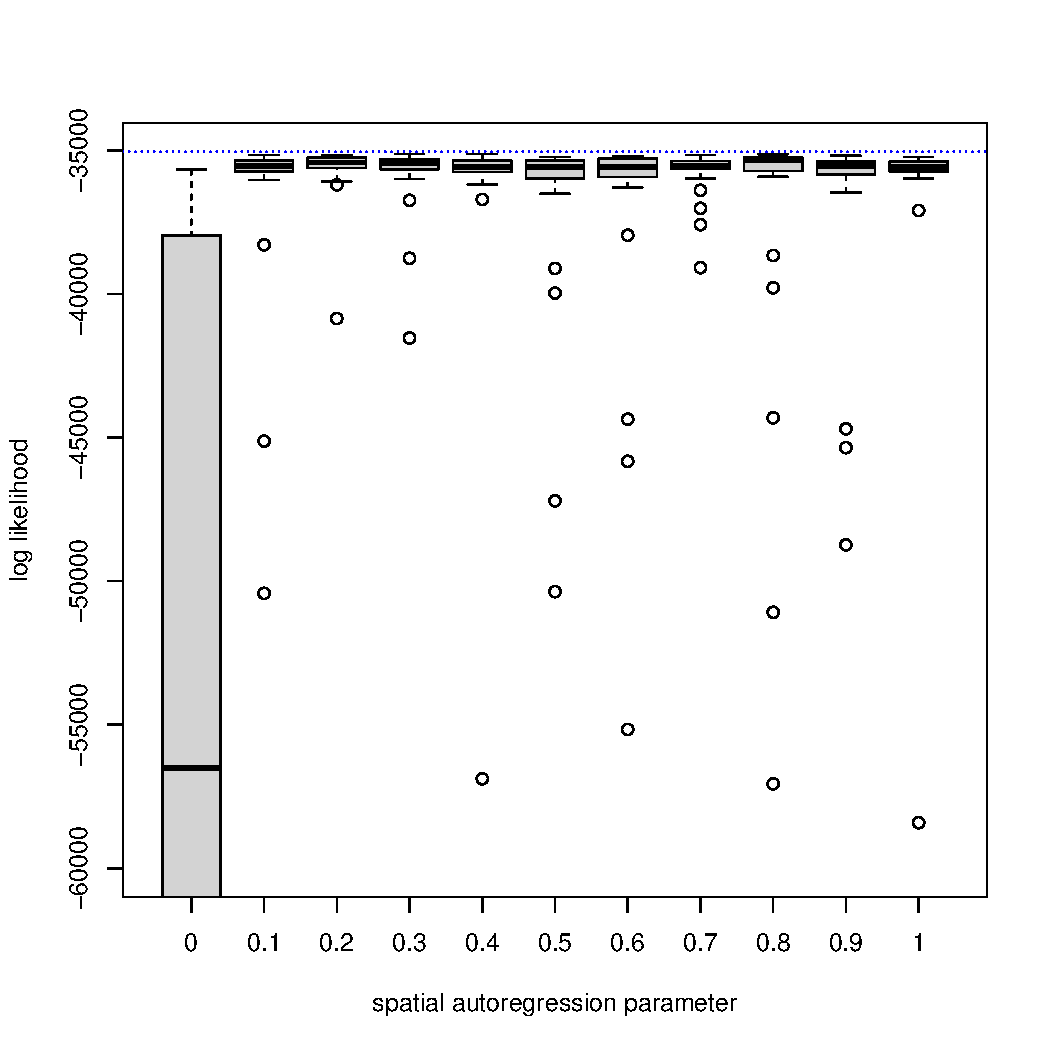
\includegraphics[width=8.5cm]{ibpf/boxplot-spat-reg.pdf}

\end{center}

\vspace{-2mm}
  
\end{frame}

\begin{frame}{Random perturbations must be smaller to match larger number  $(20\times 13)$ of parameters}
    
\vspace{-10mm}

\begin{center}
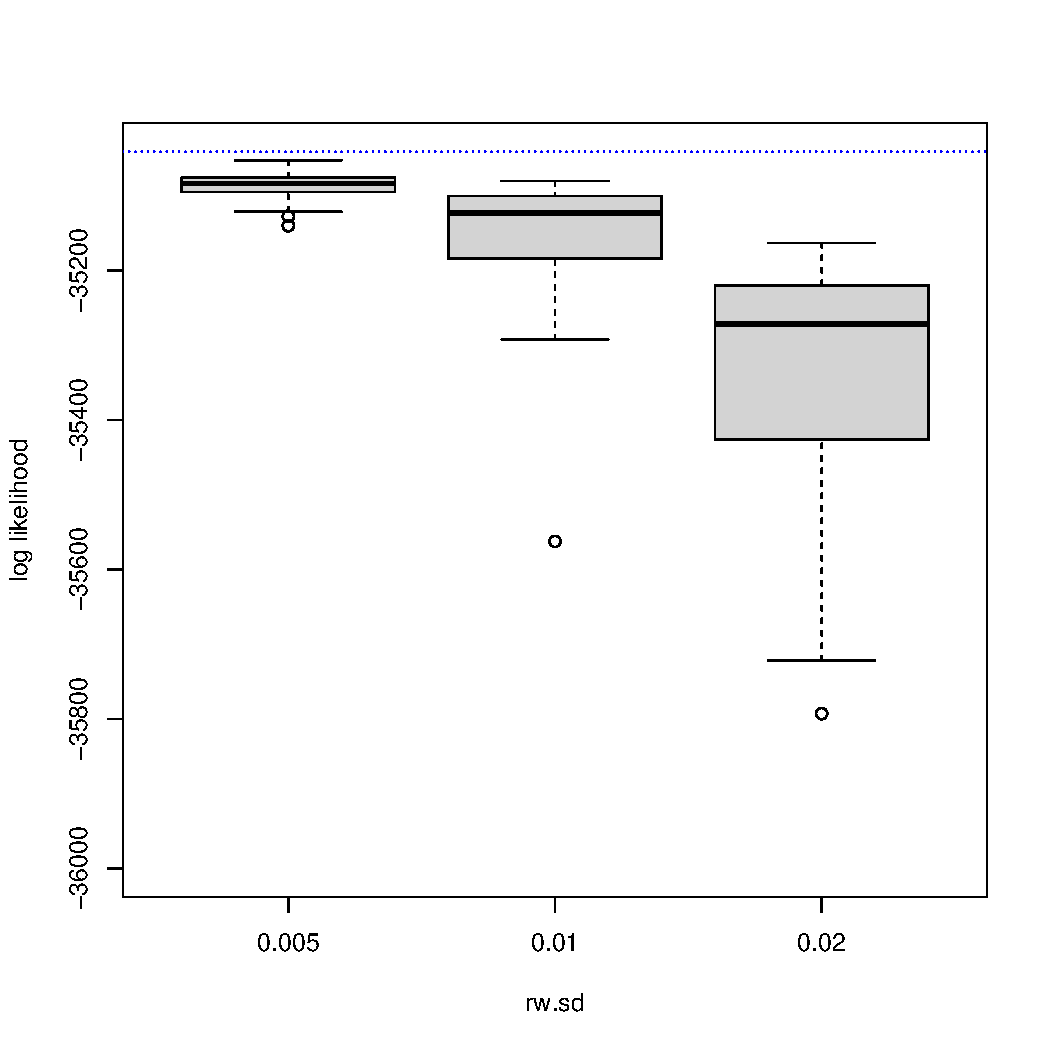
\includegraphics[width=8.5cm]{ibpf/boxplot-rw-sd.pdf}

\end{center}

\vspace{-2mm}
  
\end{frame}

\begin{frame}{Likelihood on benchmark problems with 20 towns}

  %% results: see v8-analysis, x4_analysis and x6-analysis
  
\begin{tabular}{l|rrr}
  &   Simulation & UK measles & $p$\\
  \hline
Benchmark & -35041 & -40345 & \\ 
4/13 parameters unit-specific & -35052 & -43069 & $4\times 20+9$\\
12 parameters unit-specific & -35115 & -40641& $12\times 20+1$\\

\end{tabular}

\vspace{4mm}
\bi
\item Simulated data: benchmark is likelihood at truth. Optimization used 10hr on one node.
\item Actual data: benchmark is likelihood from uncoupled model with all parameters unit-specific, and a parameter for immigration rate of new cases. Optimization used $2\times 10$hr on one node.

  \ei

  \end{frame}


\begin{frame}{Future work}

  \newcommand\futuresep{\vspace{3mm}}
  
  \begin{myitemize}
  \item We are getting close to the point where we can carry out likelihood-based inference for a flexible class of metapopulation models for measles.
Flexibility supports generation and testing of scientific hypotheses.
        
    \futuresep
    
  \item Measles was previously a motivating model system for POMP methods for single populations.

    \futuresep
    
    \item Many systems in ecology, epidemiology and elsewhere could be studied in a SpatPOMP framework.
    
\end{myitemize}

\end{frame}

\nocite{bjornstad01,grenfell04,breto19,rebeschini15,ng02,ionides21}

\begin{frame}[allowframebreaks]
\frametitle{References}
\bibliographystyle{apalike}
\bibliography{bib-sweden}
\end{frame}

%%% extra material

\begin{frame}
\frametitle{Filtering $U$-dimensional correlated Brownian motion}

\vspace{-3mm}

\begin{center}
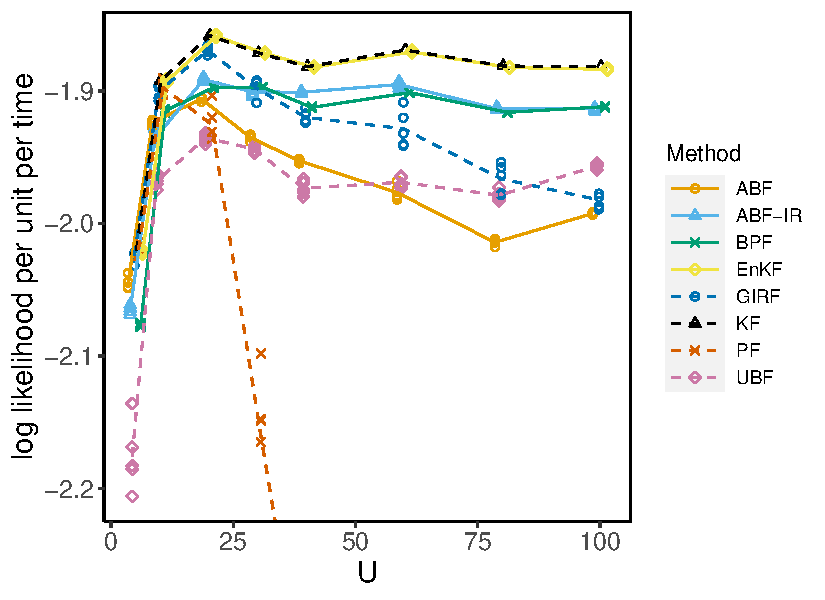
\includegraphics[width=10cm]{bm_alt_plot-1.pdf}

\vspace{-1mm}

$\cov\big(X_{\unit,\time}-X_{\unit,\time-1},X_{\altUnit,\time}-X_{\altUnit,\time-1}\big) \sim 0.4^{|\unit-\altUnit|}_{}$

\end{center}

\end{frame}



\begin{frame}
\frametitle{Filtering $U$ units of Lorenz 96 toy atmospheric model} 

\vspace{-3mm}

\begin{center}
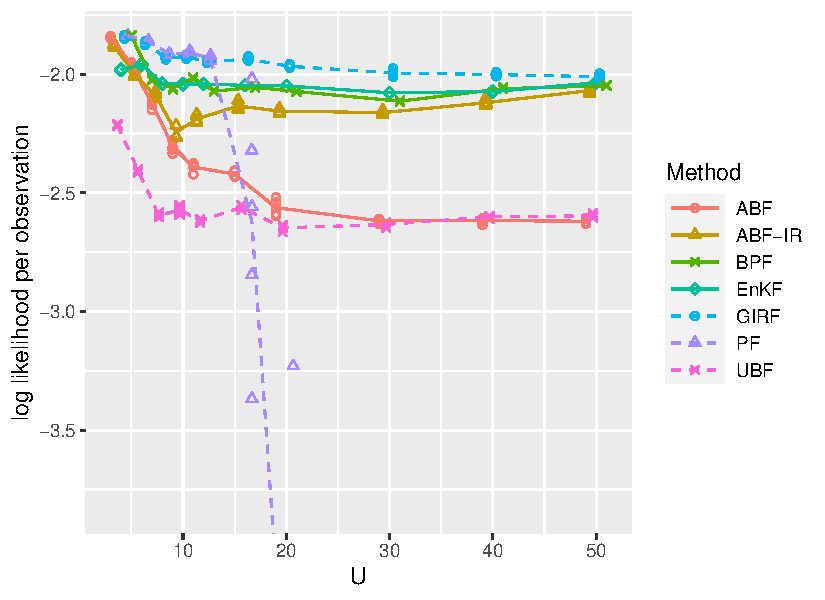
\includegraphics[width=10cm]{lz_loglik_plot-1.pdf}

\vspace{-1mm}

$dX_{\unit}(t) = \big \{  X_{\unit-1}(t) \big(X_{\unit+1}(t) - X_{\unit-2}(t)\big) - X_{\unit}(t) + F \big\} dt + \sigma \, dB_{\unit}(t)$

\end{center}

\end{frame}

\end{document}
